\section{Theory}
\label{sec:theory}
The aim of this experiment is to record the absoption spectrum
of rubidium. Therefore a diode laser is adjusted and aimed towards a cell
filled with rubidum.
The following sections introduce the theory
important for the understanding of the experiment.

\subsection{Laser basics}
\label{subsec:Laser}
A Laser (Light Amplification by Stimulated Emission of radiation)
emits highly intensive light with a long coherece length.
First of all the interaction of a radiation field with
an energy level system is considered. These includes
absorption and spontaneous and stimulated emission
of a photon, shown in figure \ref{fig:ab_em}.
\begin{figure}
\centering
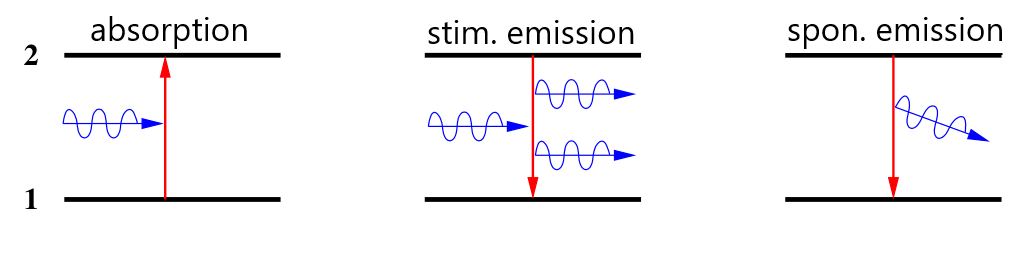
\includegraphics[width=0.7\textwidth]{ab_und_emiss.png}
\caption{Absorption and both spontaneous and stimulated emission of a photon in a two energy level system.
\cite{V61}}
\label{fig:ab_em}
\end{figure}
Absorption describes the process where a photon annihilates and
delivers energy for the transition
to a higher energy level.
Spontaneous emission discribes the opposite, a photon is
emitted, if a transition to a lower energy
level occurs spontaneously.
But most important for a laser, as the name indicates,
is the stimulated emission.
The process of stimulated emission works as follows.
If a photon with the energy same as
the energy gap between the two energy levels
encounters an excited state, another photon with
same energy and phase is emmitted and the excited state
returns to the ground state.
To run a laser, stimulated emission must be the most common interaction.
Since the occupation of the energy levels for fermions follows
the Fermi-Dirac statistics, % vielleicht doch hier noch von bolzmannstatistik sprechen
levels above the Fermi energy are
less occupied. By increasing the temperature, only
a same occupation can be accomplished.
However, this is not enough in order to ensure mostly stimulated emission.
Therefore a population inversion
between ground state and an excited
state is necessary. As to achieve this at least
a three level system is of need.
Transitions between the levels can be radiative as explained above
aswell as non radative for example in the form of lattice vibration.
Further the energy levels vary with regard
to the decay rate. In figure \ref{fig:3_n} the process of pumping and stimulated emission
is displayed for a three energy level system.
\begin{figure}
  \centering
  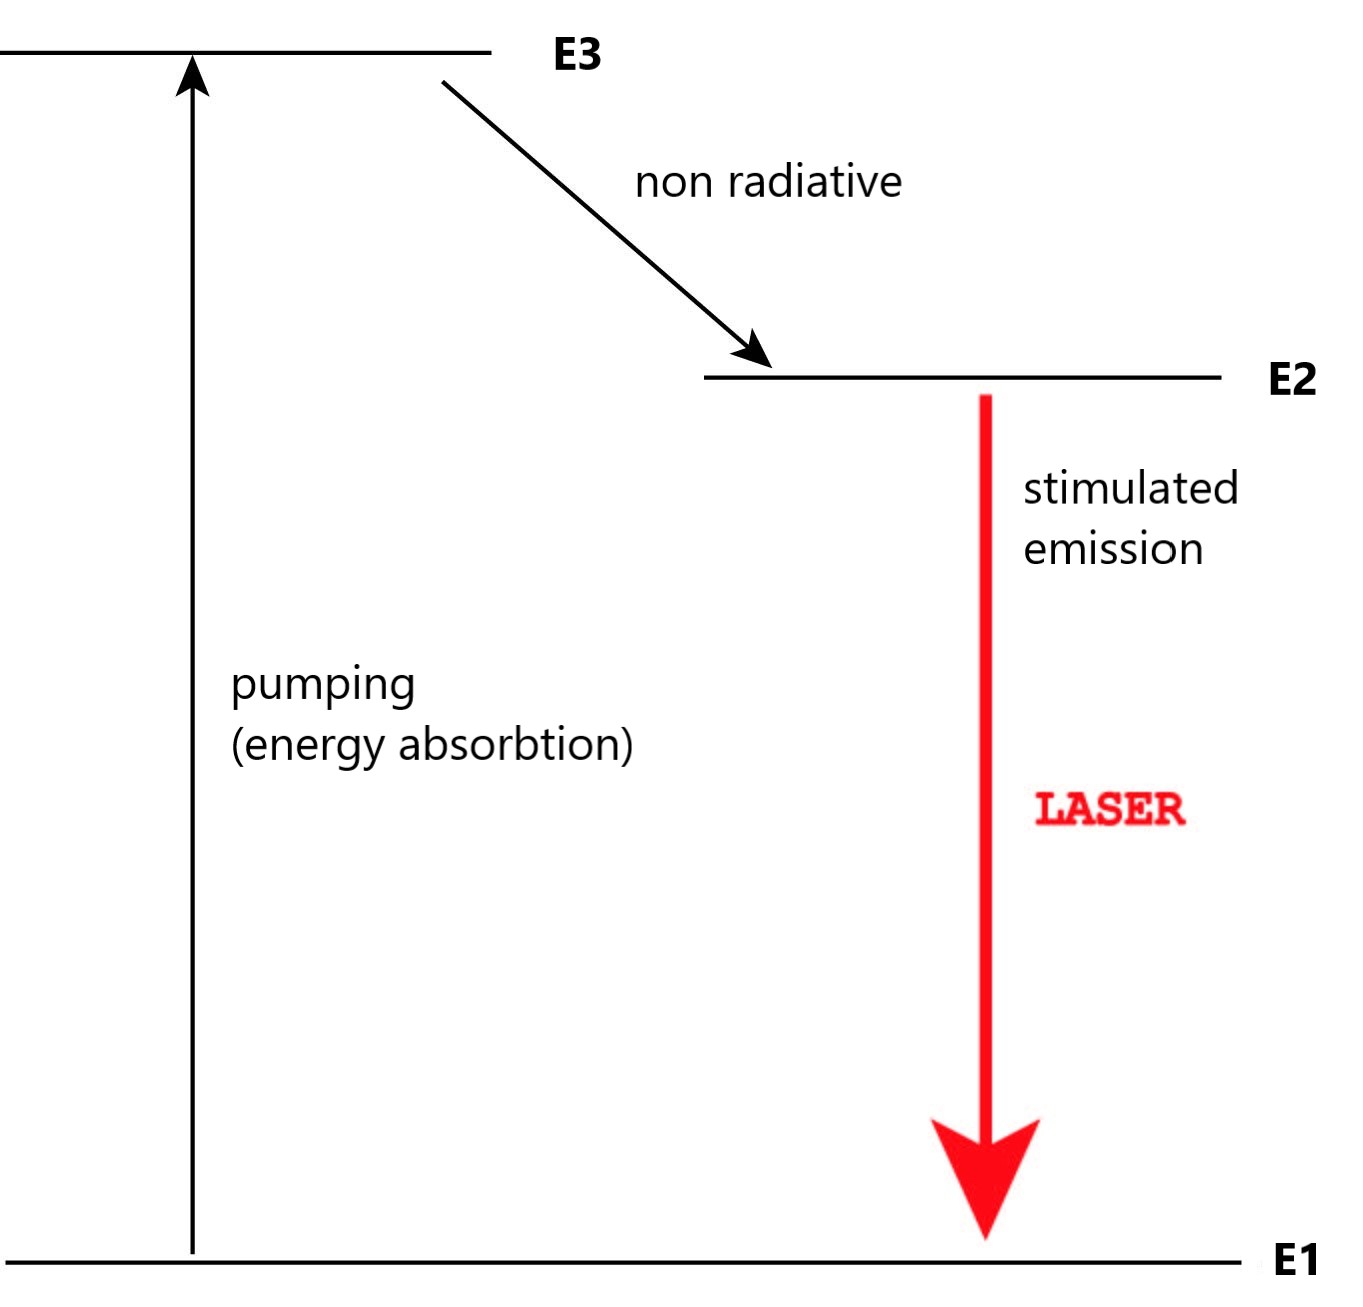
\includegraphics[width=0.4\textwidth]{Laser_3_Niveau.jpg}
  \caption{three energy level system}
  \label{fig:3_n}
\end{figure}
The Laser process for a three energy level system
goes as follows.
The transition from \textbf{E1} to \textbf{E3} is induced
by absoption of energy.
The level \textbf{E3} has a high
decay rate from \textbf{E3} to \textbf{E2},
so a transition happens almost instantaneous
through nonradiative spontaneous emission.
Level \textbf{E2} compared to \textbf{E3}
has a lower decay rate.
So when energy is continuous
pumped into level \textbf{E1},
the required population inversion
between the ground state \textbf{E1} and the
excited state \textbf{E2} is created.
Now a photon which is emitted spontaneously
through the radiative decay from
\textbf{E2} to \textbf{E1}
leads to
stimulated emissions of other photons,
thus a highly intensive
light with a long coherence length.

Beside the theoretical approach to
accomplish laser radiation, some other criteria
must also be met.
First of all a gain medium with the desired
energy gap is necessary, in which
a population inversion by pumping is created.
Pumping energy is supplied by light or electric current.
In addition the gain medium is bounded to a heat-sink
to dissipate residual heat, which is produced by pumping.
Furthermore a Laser cavity is required.
The Laser cavity consists of the gain medium and two
mirrors, one higly reflective and the other
partially transparent,
the output coupler.
In figure \ref{fig:laserschema}
a schematic laser with its components is displayed.
\begin{figure}
\centering
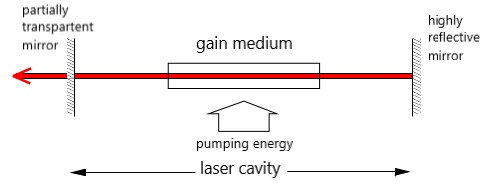
\includegraphics[width=0.7\textwidth]{laserkonzept.png}
\caption{A schematic Laser and its components.
\cite{wiki_diode}}
\label{fig:equi}
\end{figure}
The operation of the Laser cavity is as follows.
Photons are emitted through spontaneous emission
in the gain medium. The two mirrors
ensure that the photons stay in the Laser cavity
and the Laser intensity increases due to
stimulated emission of other photons.
Depending on the cavity lenght $L$,
standing waves along the cavity axis so called longituidinal modes
are developed.
The modes vary according to the wavelength and hence
the number of knots. The spacing
between frequencies of two modes in a laser
cavity is given by the free spectral range (FSR)
\begin{align}
\Delta \nu_{FSR} = \frac{c}{2Ln}
\end{align}
where $c$ is the speed of light and $n$ is
the index of refraction.
A development of transversal modes in the laser cavity
is also possible but is not discussed in detail.
The laser ray that comes out of the output coupler
contains all the frequencies of the longitudinal modes.

\subsection{Semiconductor}
\label{subsec:Semiconductor}

The diode laser is a result of the research done on semiconductors.
So first a deeper comprehension of semiconductor theory is needed.
Hence the principle funcion of a simple p-n diode is described.
A p-n diode exist out of two semiconductor materials one
n-type and the other p-type.
In the p-type semiconductor is an excess of holes
and in the n-type semiconductor, an exess of electrons.
An excess of holes or electrons can be accomplish by doping.
When n- and p-type are merged together,
electrons and holes diffuse into opposite side and recombine.
This process induces an elctric field bettween the fixed doping atoms, which
counteracts the diffusion process.
If equilibrium between the two forces is accomplished
a charge depletion zone is created
at the p-n junction.
The figure \ref{fig:equi} shows
a schematic p-n Diode in equilibrium.

\begin{figure}
\centering
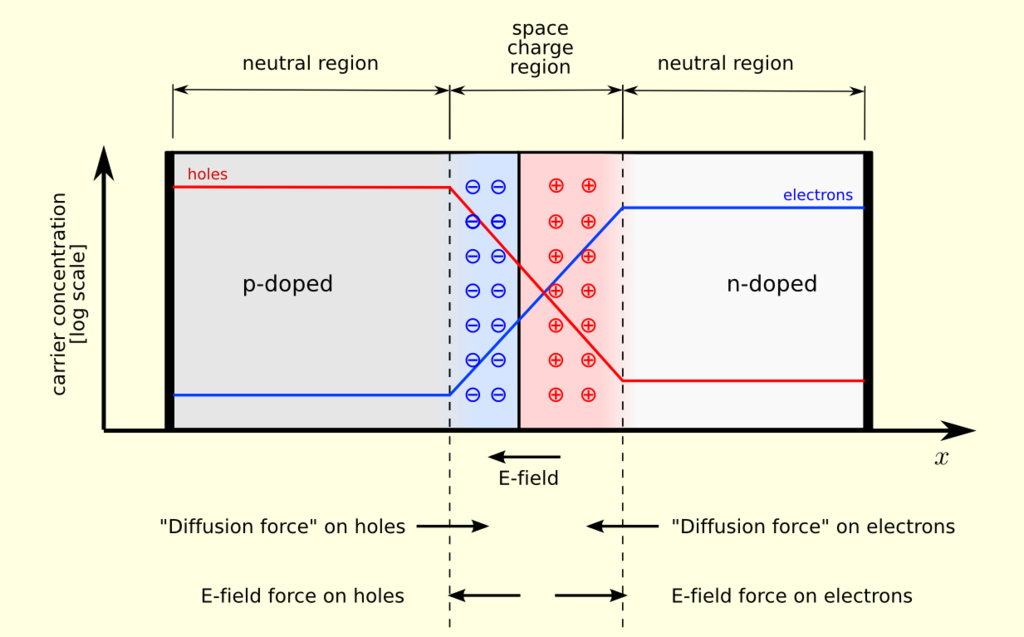
\includegraphics[width=0.7\textwidth]{equilibrium.png}
\caption{A schematic p-n Diode in equilibrium.
\cite{wiki_diode}}
\label{fig:equi}
\end{figure}

There are two possible ways to apply voltage
in forward bias and
in rewerse bias.
In forward bias the diode lets the current follow
but in the rewese bias the diode blocks the current up to the breaking point.
A typical diode characteristic is shown in figure \ref{fig:chara}
\begin{figure}
\centering
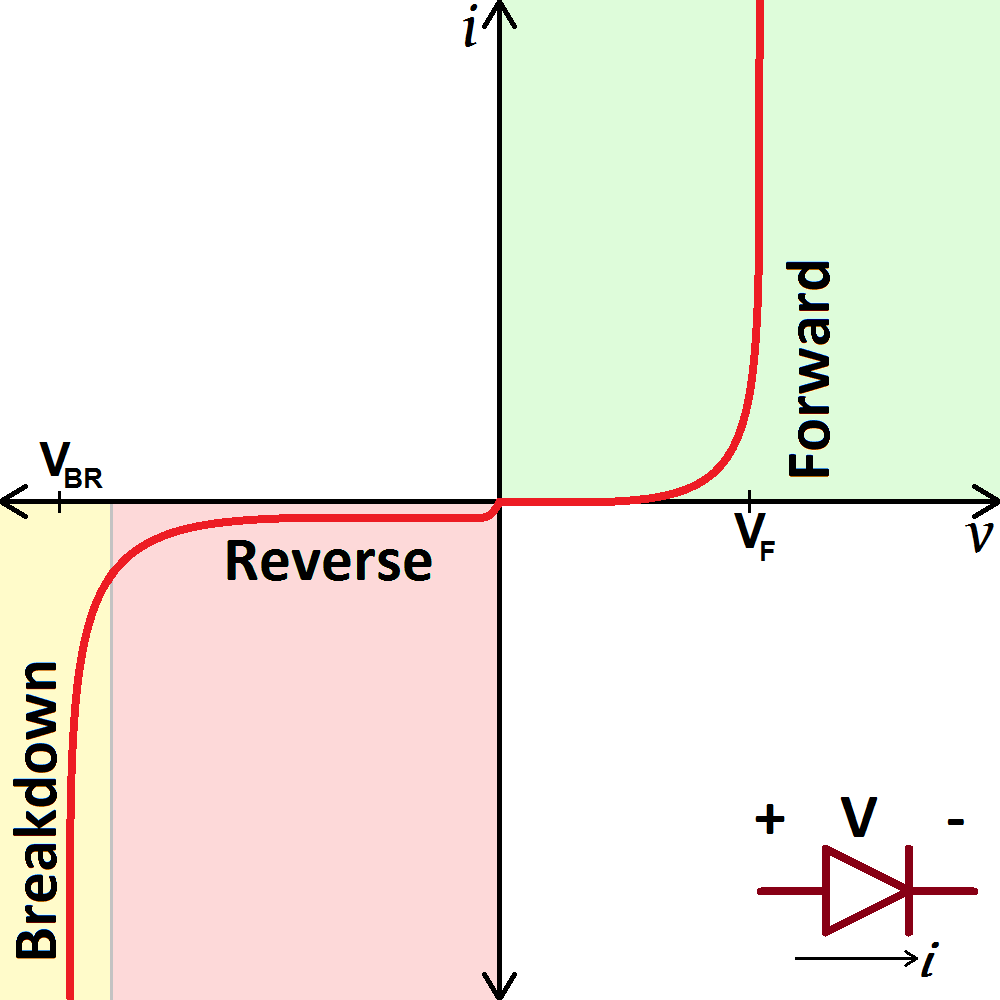
\includegraphics[width=0.5\textwidth]{Kennlinie.png}
\caption{A characteristic of a p-n Diode.
\cite{sparkfun}} % https://learn.sparkfun.com/tutorials/diodes/real-diode-characteristics
\label{fig:chara}
\end{figure}
For the Diode Laser a light-emitting diode (LED)
is necessary. A LED differs in terms of
the band gap
from a simple p-n diode.
For a LED a direct band gap is needed, so a photon
with the energy of the band gap is
emitted if electrons and holes recombine.

\subsection{Diodenlaser}
\label{subsec:diodenlaser}
By applying the informations of previous sections
a diode laser can be explained.
The diode laser consists of a special semiconductor chip.
The chip has a certain structur shown in figure \ref{fig:chip}.
\begin{figure}
  \centering
  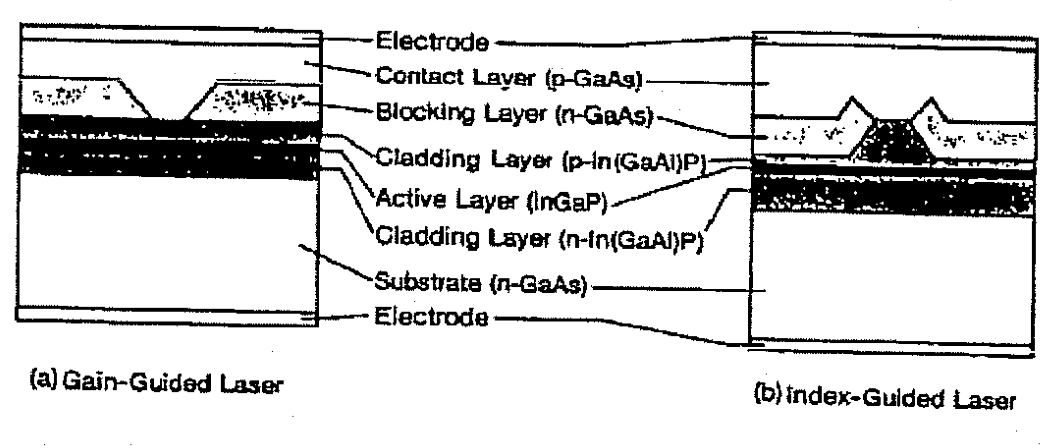
\includegraphics[width=0.7\textwidth]{chip.png}
  \caption{Two different typical structurs profiles of a diode laser chip.\cite{V61}}
  \label{fig:chip}
\end{figure}
The active layer of the chip has a higer refraction index than
its surroundings. Because of that light which is emmitted
in the active layer through recombination of electron-hole pairs
is confined in the channel by total internal reflection.
% The cleaved facets at the end of the chip
% are coated to incraese or decrease the facet reflectivity
The cavity mirrors and output couplers arise
by coating the cleaved facets at the end of the chip,
to increase or decrease the facet reflectivity.
So a tiny semiconductor laser cavity inside the chip
with a typical linewidth
$\delta \nu \approx \SI{50}{\mega\hertz}$
is developed.
A population inversion
can be achieved through current.
But at low levels of current
the optical losses are higher than the gain
so a population inversion is not achieved and
the laser diode emits a broad-band light
through spontaneous emission
like a LED.
To obtain a coherent laser beam the current must be above
a threshold current, where the gain is higher than the
optical losses, so a population inversion is created.
Futhermore the laser intensity increases linearly with
injection current.
The output beam of the chip is elliptical and strongly diverging
therefore a collimating lens is necessary.
There are still two problems to solve.
First the diode laser is very sensitive to optical feedback.
Already $10^{-6}$ of the output light affects
the stability of the frequency
when scattered back into the
laser cavity.
Therefore a diffraction grating is installed which
is shown in figure \ref{fig:aufbau}.
\begin{figure}
  \centering
  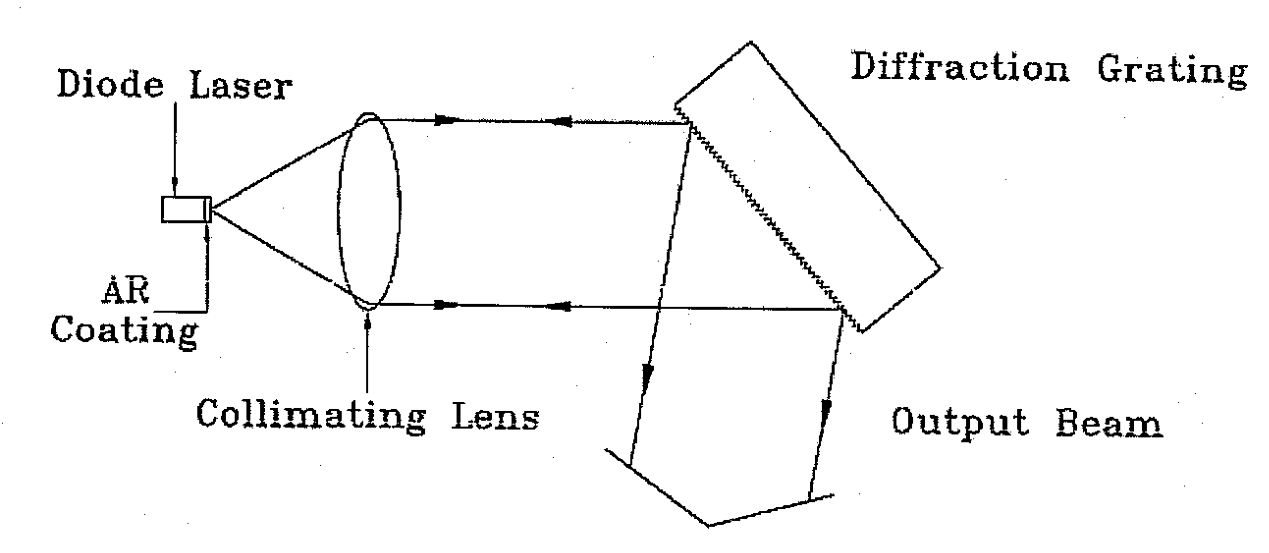
\includegraphics[width=0.7\textwidth]{aufbau.png}
  \caption{Schematical layout of a diode laser with collimating lens and diffraction grating.\cite{V61}}
  \label{fig:aufbau}
\end{figure}

The diffraction grating ensures that a majority part of
the light that is scattered back into the laser cavity is from the first order
diffraction of the grating. This leads to
a frequency-stabilized laser beam, because only certain wavelengths,
depending on the position
of the grating, scatter back in the cavity.
Most part of the light scatters in the 0. order,
the output Beam, but $\SI{15}{\percent}$ scatters back into
the cavity, which is enough to cause the stabilisation.
Futhermore the grating and the highly reflective end of the chip form a
further Laser cavity,
the so called external cavity.
??Hence the diffraction grating fortunately solves the second
problem which is the large linewidth of the bare
diode laser($\delta \nu \approx \SI{50}{\mega\hertz}$)
compared to the linewidth of atomic transitions
(here $\Gamma \approx \SI{5}{\mega\hertz}$).
The external cavity
reduces the linewidth namely to $\Delta\nu\l \SI{1}{\mega\hertz}$.
All in all the diffraction grating
functions as a controlled feedback for frequency stability
and to reduce the linewidth of the laser.


\subsection{Beiträge im Laser}
\label{subsec:}
To observe atomic transitions, precise control
of the developed frequency is necessary.
In theory the Laser operates at the mode with the highest net gain
and other modes do not occur.
However in reality it is possible, that multiple modes occur, leading
to spectrum of multiple frequencies. In the following the focus will
lay on single mode operation, since this is the desired case
for the experiment.

As shown in figure \ref{fig:gain_overview} the main contributions
to the \textbf{net gain} can be reduced to
the \textbf{medium}, \textbf{internal cavity}, \textbf{grating feedback}
and  \textbf{external cavity}.
The best case scenario, in which all gain functions peak at the
same wavelength, is displayed in figure \ref{fig:ideal_gain_overview}
In the following the four contributions will be explained seperately.


\FloatBarrier
\begin{figure}
  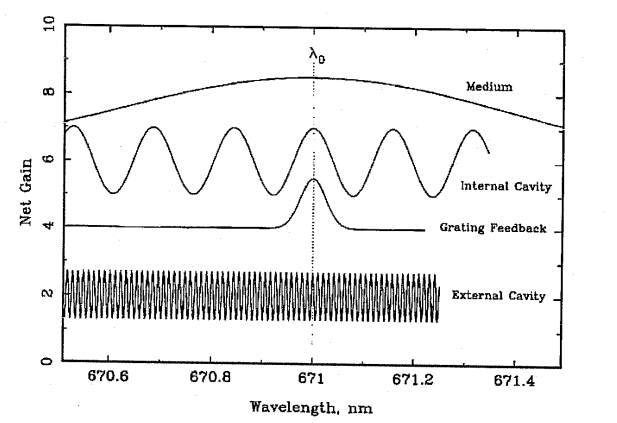
\includegraphics{gain_overview.png}
  \caption{Overview for the contributions to the net gain as function of
            wavelength.\cite{sample}}
  \label{fig:gain_overview}
\end{figure}
\FloatBarrier

\FloatBarrier
\begin{figure}
  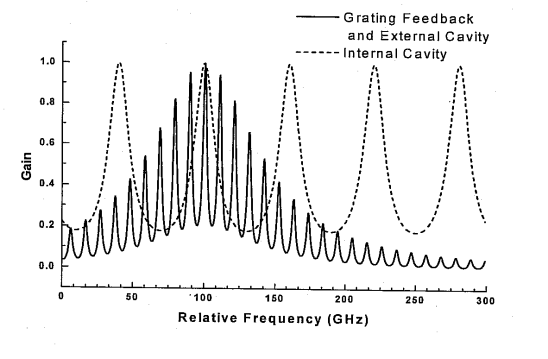
\includegraphics{ideal_gain_overview.png}
  \caption{Overview for the contributions to the net gain as function of
            wavelength in the ideal case.\cite{sample}}
  \label{fig:ideal_gain_overview}
\end{figure}
\FloatBarrier


\paragraph{Medium gain}
The medium gain as function of frequency(or wavelength) has
the shape of a broad peak and is determined by two parameters.
The band gap of the laser's semiconductor material and the temperature
at which the laser is used. Since the band gap is a fixed
quantity, the medium gain can only be controlled by changing
the temperature, which changes the peak's position.
The relation between output wavelength and
temperature is graphically shown
in figure \ref{fig:medium_gain_temperature.png}
for multiple modes.



\paragraph{Internal cavity}
As described in \ref{subsec:diodenlaser} the diode junction itself
acts as a laser cavity, that is referred to as the \textbf{internal cavity}.
The associated contribution to the gain is periodically dependent on
the frequency or the wavelength respectively. The \textbf{FSR} is about
$\Delta\nu_{\text{FSR}} = \SI{60}{\giga\hertz}$ (or
$\Delta\lambda = \SI{0.122}{\nano\meter}$ respectively).
Since the laser's output wavelength shows a linear
temperature dependency(see figure \ref{fig:medium_gain_temperature}),
the gain function for the internal cavity is moved in frequency$/$wavelength.
A change in temperature is for example evoked by the diode current,
that will increase the temperature faster($\sim \SI{1}{\micro\second}$),
as if the laser is heated externally($\sim \SI{10}{\second}$).
Besides heating the laser, the diode current changes the optical
path length in the diode junction, by manipulating the concentration
of charge carriers. Due to this the frequency is increased at a rate of
approximately $\SI{200}{\mega\hertz\per\milli\ampere}$, until it reaches
its maximum at around $\mathcal{O}(\SI{1}{\giga\hertz})$.
This effect is illustrated by figure \ref{fig:injectioncurrent_wavelength}.


Since the gain function of the laser medium and the gain function of
the internal cavity are not moved in the same way by a change in temperature,
a problem named \textbf{mode hops} can occur. This is the case,
when the laser's mode changes, because the overall gain maximum
switches from one peak of the internal cavity
gain function (see figure \ref{fig:gain_overview}) to another.



\paragraph{Grating feedback}
With the diffraction grating, light with a specific wavelength
can be scattered back into the laser. This allows one to precisely
influence the gain function. By modifying the left/right angle
it is possible to choose which wavelengths are scattered back.
By modifying the up/down angle, the order of diffraction, that
is scattered back, is chosen. In this case the grating
should be configured in a way, that mostly light from
the first order is send back. Figure \ref{gain_overview}
displays the small wavelength-band that can be chosen with
the grating feedback. Hence it is possible to deal with "mode hopping"
by changing the left/right angle of the grating. This is illustrated
in figure \ref{fig:mode_hops}


\FloatBarrier
\begin{figure}
  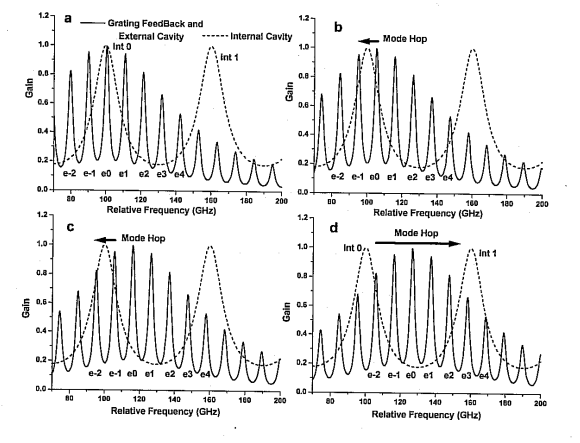
\includegraphics{mode_hops.png}
  \caption{Illustration of mode hopping, due to change in grating feedback and external cavity.\cite{sample}}
  \label{fig:mode_hops}
\end{figure}
\FloatBarrier


-Littrow configuration (?)


\paragraph{External cavity}
The Grating and the reflective back of the diode form another
cavity. It is reffered to as the \textbf{external cavity}.
The external cavity posseses a by far greater length then
the internal one, which results into a
smaller FSR of
$\sim \SI{10}{\giga\hertz}$(in the case of $L = \SI{15}{\milli\meter}$).
If the laser itself is not moved, the gain function
contribution of the external is only shifted if the grating
is moved. In the experiment the grating's position
is periodically changed by a \textbf{piezzo element} or chaning the left/right angle of the grating.







\FloatBarrier
\begin{figure}
    \centering
  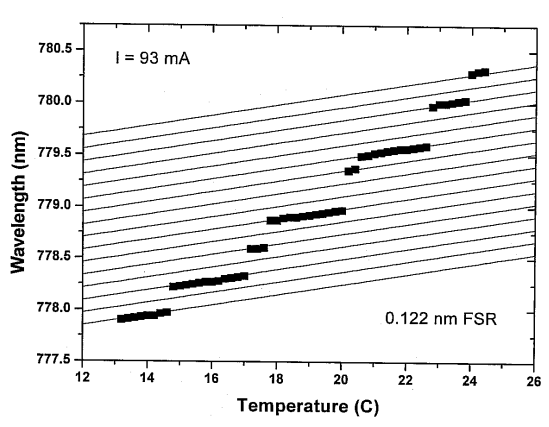
\includegraphics{medium_gain_temperature.png}
  \caption{Relation between wavelength and diode current
           for different laser modes at a constant temperature.}
  \label{fig:medium_gain_temperature}
\end{figure}
FloatBarrier





Therefore ...


\subsection{Rubidum spektrum}
\label{subsec:}


\subsection{piezo}
\label{subsec:}
